
\documentclass[10pt,conference]{IEEEtran}
\usepackage{color}
\usepackage{url}
\usepackage{graphicx}
%\usepackage{cite}
\usepackage[square, sort&compress, numbers]{natbib}
\renewcommand{\bibfont}{\footnotesize}
\usepackage{amsmath}
\usepackage{listings}
\usepackage{enumerate}
\usepackage{lipsum}
\usepackage{textcomp}
\usepackage[caption=false,font=footnotesize]{subfig}
\usepackage[table]{xcolor}
%\usepackage[square, comma, sort&compress]{natbib}
\definecolor{light-gray}{gray}{0.80}
\DeclareMathSizes{8}{8}{8}{8}
\usepackage{authblk}

\begin{document}
%\title{Behavioral Analysis of the Agent-Based Community Grid Solution for the Large Hadron Collider beauty Experiment}
\title{Using Model Checking to Analyze the System Behavior of the LHC Production Grid}
\author[1,3]{Daniela Remenska}
\author[2]{Tim A.C. Willemse}
\author[1]{Kees Verstoep}
\author[1]{Wan Fokkink}
\author[3]{Jeff Templon}
\author[1]{Henri Bal}

\affil[1]{Dept. of Computer Science, VU University Amsterdam, The Netherlands}
\affil[2]{Dept. of Computer Science, TU Eindhoven, The Netherlands}
\affil[3]{NIKHEF, Amsterdam, The Netherlands}

\maketitle

\begin{abstract}
DIRAC (Distributed Infrastructure with Remote Agent Control) is the grid
solution designed to support production activities as well as user data analysis
for the Large Hadron Collider ``beauty'' experiment. It consists of cooperating
distributed services and a plethora of light-weight agents delivering the
workload to the grid resources.  Services accept requests from agents and
running jobs, while agents actively fulfill specific goals. Services maintain
database back-ends to store dynamic state information of entities such as jobs,
queues, or requests for data transfer. Agents continuously check for changes in the
service states, and react to these accordingly. The logic of each agent is
rather simple; the main source of complexity lies in their cooperation. These
agents run concurrently, and communicate using the services' databases as a
shared memory for synchronizing the state transitions. Despite the effort
invested in making DIRAC reliable, entities occasionally get into inconsistent
states. Tracing and fixing such behaviors is difficult, given the inherent
parallelism among the distributed components and the size of the
implementation.

In this paper we present an analysis of DIRAC with mCRL2, process algebra with
data. We have reverse engineered two critical and related DIRAC subsystems, and
subsequently modeled their behavior with the mCRL2 toolset. This enabled us to
easily locate race conditions and livelocks which were confirmed to occur in the
real system. We further formalized and verified several behavioral properties of
the two modeled subsystems.
\end{abstract}

\section{Introduction}

The Large Hadron Collider beauty (LHCb) experiment \cite{LHCb} is one of the
four large
experiments conducted on the Large Hadron Collider (LHC) accelerator, built by
the European Organization for Nuclear Research (CERN). Immense amounts of data
are produced at the LHC accelerator, and subsequently processed by physics
groups and individuals worldwide. The sheer size of the experiment is the
motivation behind the adoption of the grid computing paradigm. The grid storage
and computing resources for the LHCb experiment are distributed across several
institutes in Europe. To cope with the complexity of processing the vast amount
of data, a complete grid solution, called DIRAC (Distributed Infrastructure with
Remote Agent Control) \cite{DIRAC_CommGridSolution,DIRAC_ReliableDataMaangement}, 
has been designed and developed for the
LHCb
community.

DIRAC forms a layer between the LHCb user community and the heterogeneous
grid resources, in order to allow for optimal and reliable usage of these
resources. It consists of many cooperating distributed services and light-weight
agents which deliver the workload to the resources. The logic of each individual
component is relatively simple; the overall system complexity emerges from the
cooperation among them. Namely, these agents run concurrently, and communicate
using the services' databases as a shared memory (blackboard paradigm \cite{IEEEexample:blackboard_systems}) for
synchronizing state transitions of various entities.

Although much effort is invested in making DIRAC reliable, entities occasionally
get into inconsistent states, leading to a potential loss of efficiency in both
resource usage and manpower. Debugging and fixing the root of such encountered
behaviors becomes a formidable mission due to multiple factors: the inherent
parallelism present among the system components deployed on different physical
machines, the size of the implementation ($\sim$150,000 lines of Python code),
and the distributed knowledge of different subsystems within the collaboration.

In this paper we propose the use of rigorous (formal) methods for improving
software quality. Model checking \cite{ProcessesWithData} is one such technique for analysis of an
abstract model of a system, and verification of certain system properties of
interest. Unlike conventional testing, it allows full control over the execution
of parallel processes and also supports automated exhaustive state-space
exploration. We used the mCRL2 language \cite{FormalLanguagemCRL2} and toolset \cite{mCRL2Toolset} to model the behavior of two
critical and related DIRAC components: the Workload Management (WMS) and the
Storage Management System (SMS). Based on Algebra of Communicating Processes
(ACP) \cite{process_algebra}, mCRL2 is able to deal with generic data types as well as user-defined
functions for data transformation. This makes it particularly suitable for
modeling the data manipulations made by DIRAC's agents. Visualizing the state
space and replaying scenarios with the toolkit's simulator enabled us to gain
insight into the system behavior and incrementally improve the model. 
Already using these techniques, critical race-conditions and livelocks were detected and confirmed to
occur in the real system. Some of them were a result of simple coding bugs;
others unveiled more elementary design problems. We further formulated,
formalized and verified several application-specific properties.

The idea of modeling existing systems using 
formal techniques is as such not new. Earlier studies
(\cite{SPIN_case_study,desing_validation_protocols,protocol_verification_muCRL,SLAMToolkit,SlidingWindowProtocol,DHCP_SPIN}) mostly focused
on modeling and verifying hardware or communication protocols, since
the formal languages and tools at hand were not sufficiently mature
to cope with more complex data-intensive distributed systems. More
recently, success stories on modeling real-life concurrent systems with
data have been reported (\cite{CMS_LHC, Linux_driver,verstoep_et_al, SystemC_processAlgebra}).
Tools for automatic translation of the system implementation language into
 formal language constructs can greatly
simplify the analysis. However, this has so far been feasible only when the
language of implementation is domain-specific, or alternatively, a
reasonably small subset of a general-purpose language is considered for
translation. 

We believe that the challenges and results of this work are unique in
a number of aspects. First, to the best of our knowledge, the code-base
and the number of concurrent grid components engaged in providing DIRAC's
functionality considerably outnumber most of the previous industrial cases. Second,
the choice of Python as implementation platform has led to the prevailing
usage of dynamic structures (whose types and sizes are determined at
runtime) throughout DIRAC, challenging the transition to an abstract
formal representation. We have established general
guidelines on extracting a model outline from the implementation. These
can be reused in many distributed systems to address concurrency issues arising 
from the use of shared storage for inter-process communication. Third,
analysis of this kind is typically performed after a problem has already
surfaced in the real system, as a means to understand the events which
led to it and test for possible solutions. We managed to come across an
actual bug at the same time it was observed in practice, which increased
our confidence in the soundness of the model.

The paper is organized as follows. Section 2 introduces the architecture
of DIRAC, focusing on the two subsystems chosen as case studies. Section 3 gives a brief
overview of the mCRL2 language, and describes our approach to abstracting
and modeling the behavior of these subsystems. Section 4 presents the
analysis with the mCRL2 toolset and the issues detected. Section 5
concludes. 

\section{DIRAC: A Community Grid Solution}
\label{sec:Section_2}
\subsection{Architecture Overview}

The development of DIRAC started in 2002 as a system for production of simulation
data that would serve to verify physics theory, aspects of the LHCb detector design, as
well as to optimize physics algorithms. It gradually evolved into a complete community
grid solution for data and job management, based on a general-purpose framework
that can be reused by other communities besides LHCb. Today, it covers all major
LHCb tasks starting with the raw data transfer from the experiment's detector to
the grid storage, several steps of data processing, up to the final user
analysis. 
It provides a concurrent use of over 60K CPUs and 10M file replicas distributed over
tens of grid sites. The community of users has grown to several hundreds, loading the 
LHC grid resources with up to 50K simultaneously running jobs during peak processing periods.
Python was chosen as the implementation language, since it enables
rapid prototyping and development of new features. DIRAC follows the Service
Oriented Architecture (SOA) paradigm, accompanied by a network of lightweight
distributed agents which animate the system. Its main components are depicted in
Fig.~\ref{fig:DIRAC-Arch}. 

\begin{figure}[t]
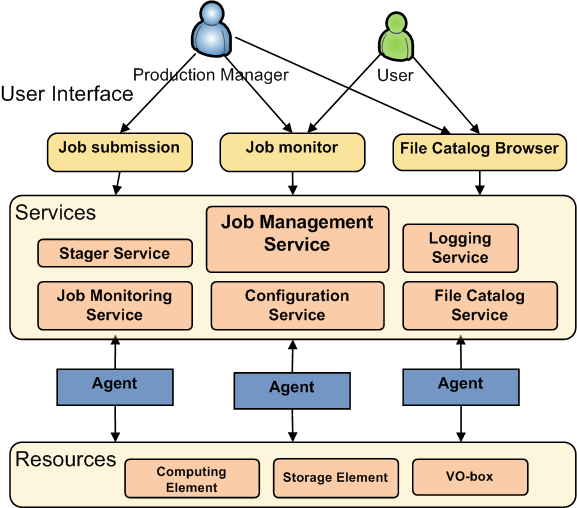
\includegraphics[width=0.85\linewidth,keepaspectratio=true]{./DIRAC_Architecture.png}
\centering
\caption{DIRAC Architecture overview}
\vspace{-5 pt}
\label{fig:DIRAC-Arch}
\end{figure}

The \textit{services} are passive components that react to requests from their clients,
possibly soliciting other services in order to fulfill the requests. They run as
permanent processes deployed on a number of high-availability hosts (VO-boxes)
at CERN, and store the dynamic system state information in database
repositories. The user interfaces, agents or running jobs can act as clients
placing the requests to DIRAC's services.

\textit{Agents} are active components that fulfill a limited number of specific system
functions. They can run in different environments, depending on their mission.
Some are deployed close to the corresponding services, while others run on the
grid worker nodes.  Examples of the latter are the so-called Pilot Agents, part
of the Workload Management System explained in the following section. All DIRAC
agents repeat the same logic in each iteration cycle: they monitor the service states,
 and respond by initiating actions (like job
submission or data transfer) which may update the states of various system
entities.

\textit{Resources} are software abstractions of the underlying heterogeneous grid
computing and storage entities allocated to LHCb, providing a uniform interface
for access. The physical resources are controlled by the site managers and made
available through middleware services such as gLite \cite{gLite}.

The DIRAC functionality is exposed to users and developers through a rich set of
command-line tools forming the DIRAC API, complemented by a Web portal for
visually monitoring  the system behavior and controlling the ongoing tasks. Both
the Web and command-line \textit{interfaces} ensure secure system access using X509
certificates. 

In the following, we focus on two related subsystems that are considered the backbone of DIRAC. These
are the ones where problematic state changes are most often encountered,
 which are difficult to trace and correct. Understanding their behavior 
is essential for interpreting the issues that were discovered during the model analysis and verification.

\subsection{Workload Management System}

The driving force of DIRAC is the Workload Management System (WMS). Taking into
account the heterogeneous, dynamic, and high-latency nature of the distributed computing environment, a
\textit{Pilot Job paradigm}, illustrated in Fig.~\ref{fig:DIRAC-WMS}, was chosen as an efficient way to
implement a pull scheduling mechanism.  Pilot jobs are simply resource
reservation processes without an actual payload defined a priori. They are
submitted to the grid worker nodes with the aim of checking the sanity of the
operational environment just before pulling and executing the real payload. This
hides the fragility of the underlying resources and increases the job success
rate, from the perspective of end users. Centralized \textit{Task Queues} contain all the
pending jobs, organized in groups according to their requirements. This enables
efficient application of job priorities, enforcing fair-share policies and
quotas, which are decided within the LHCb community, without the need of any
effort from the grid sites.  
\begin{figure}[b]
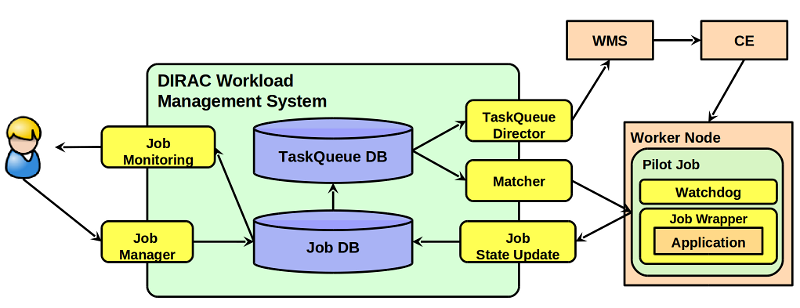
\includegraphics[width=\linewidth,keepaspectratio=true]{./DIRAC_WMS1.png}
\centering
\caption{DIRAC Workload Management System \cite{DIRAC_pilot_WMS}}
\vspace{-5 pt}
\label{fig:DIRAC-WMS}
\end{figure}
 
The basic flowchart describing the evolution of a job's states is depicted in
Fig.~\ref{fig:DIRAC-job-state-machine}. After submission through the \textit{Job Manager} (``Received''), the complete
job description is placed in the DIRAC job repository (the Job DB). Before jobs
become eligible for execution, a chain of optimizer agents checks and prioritizes
them in queues, utilizing the parameters information from the Job DB.
\begin{figure}[t]
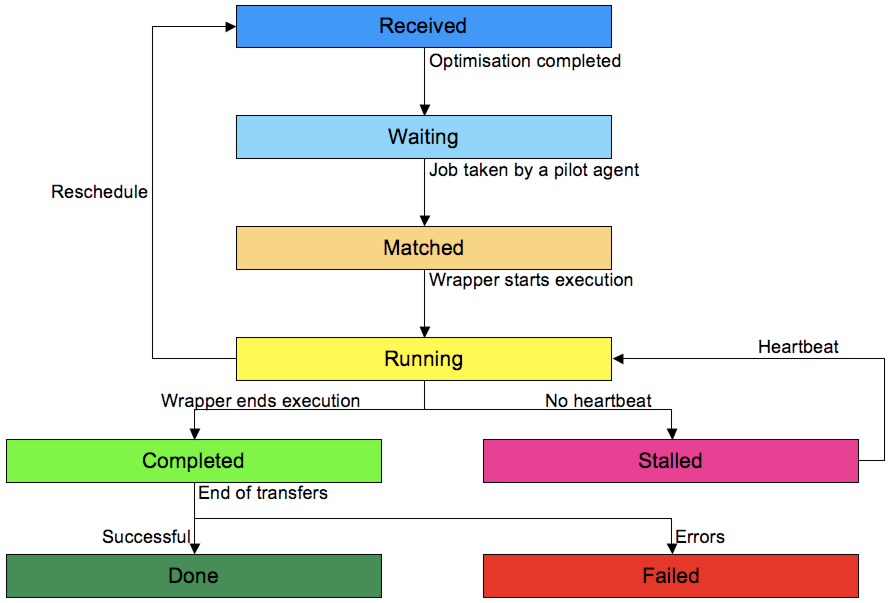
\includegraphics[width=\linewidth,keepaspectratio=true]{./dirac-primary-states.png}
\centering
\caption{Job state machine \cite{ProductionShifterGuide}}
\label{fig:DIRAC-job-state-machine}
\vspace{-5 pt}
\end{figure} 
If the requested data resides on tape storage, the \textit{Job
Scheduling Agent} will pass the control to a specialized \textit{Stager} service (part of
the SMS explained in the next section), before placing the job in a Task Queue
(``Waiting''). Based on the complete list of pending payloads, a specialized \textit{Task
Queue Director} agent submits pilots to the computing resources via the available job
submission middleware (e.g., gLite WMS). After
a \textit{Matcher} service pulls the most suitable payload for a pilot (``Matched''), a \textit{Job
Wrapper} object is created on the worker node, responsible for retrieving the
input sandbox, performing software availability checks, executing the actual
payload on the worker node (``Running''), and finally uploading any output data
necessary (``Done'' or ``Failed''). The wrapper can catch any failure exit state
reported by the running physics applications. At the same time, a \textit{Watchdog}
process is instantiated to monitor the behavior of the Job Wrapper and send
heartbeat signals to the monitoring service. It can also take actions in case
resources are soon to be exhausted, the payload stalls, or a management command
for killing the payload is received.

Although the grid storage resources are limited, it is essential to keep all
data collected throughout the experiment's run. Tape backends provide a reliable
and cheap solution for data storage. The additional workflow step 
necessary for input data files residing on tape is carried out inside the
Storage Management System (SMS).

\subsection{Storage Management System}

The DIRAC SMS provides the logic for pre-staging files from tape to a disk cache
frontend, before a job is able to process them. Smooth functioning of this
system is essential for production activities which involve reprocessing 
older data with improved physics software, and happens typically several times
per year.

A simplified view of the system is shown in  Fig.~\ref{fig:DIRAC-SMS}. The workflow is initiated
with the \textit{Job Scheduling Agent} detecting that a job is assigned to process files
only available on tape storage. It sends a request for staging (i.e., creating a
cached replica) to the \textit{Storage Manager Handler} service with the
list of files and a callback method to be invoked when the request has been
processed. The Storage Management DB is immediately populated with records which
are processed by a sequence of agents in an organized fashion. The relevant
tables in the SMS DB are the \textit{Tasks} and \textit{CacheReplicas}, whose
entities maintain a state observed and updated by these agents. \textit{Tasks} maintain
general information about every job requesting a service from the SMS. The
details about every file (i.e., the Storage Element where it resides, the
size, checksum, number of tasks that requested it), are kept in the \textit{CacheReplicas}
table. Other auxiliary tables maintain the relationship between these entities.
\begin{figure}[t]
\begin{center}
 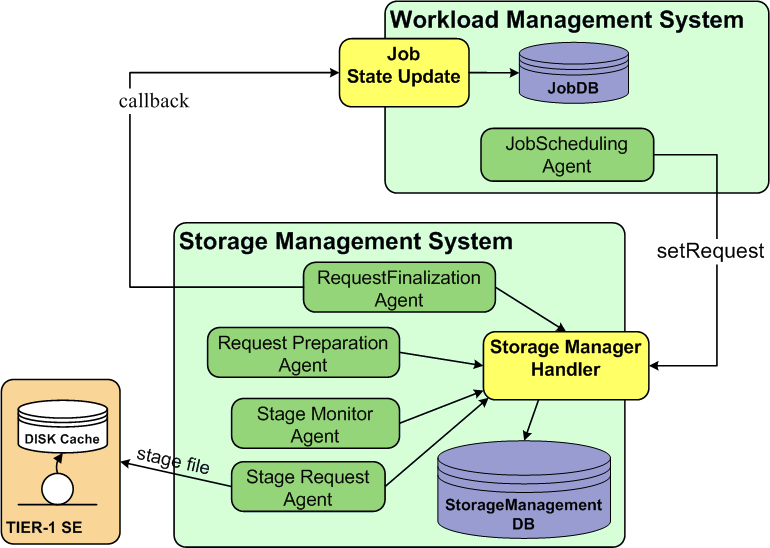
\includegraphics[width=0.9\linewidth,keepaspectratio=true]{./SMS_simplified.png}
\end{center}
\caption{DIRAC Storage Management System}
\vspace{-15 pt}
\label{fig:DIRAC-SMS}
\end{figure}

The processing begins with the \textit{Request Preparation Agent}. It selects all the
``New'' replica entries, checks whether they are registered in a Logical
File Catalog (LFC), and retrieves their metadata. In case of problematic catalog
entries, it can update the state of the \textit{CacheReplicas} and the related \textit{Tasks}
entries to ``Failed''. Non-problematic files are updated to a
``Waiting'' state. The \textit{Stage Request Agent} is responsible for placing the actual staging
requests for all ``Waiting'' entries, via dedicated storage middleware that
communicates with the tape backends. These requests are grouped by Storage Element (SE) prior to
submission, and carry information about the requested (pin) lifetime of the
replicas to be cached. If certain pathologies are discovered (i.e., lost,
unavailable, or zero-sized files on tape), it can update the corresponding
entries to ``Failed'' in a similar manner. Otherwise, they are promoted to
``StageSubmitted''. The agent responsible for monitoring the status of submitted
requests is the \textit{Stage Monitor Agent}. It achieves this by interrogating the
storage middleware to see if the ``StageSubmitted'' files are successfully
replicated on disk cache. In case of success, the \textit{CacheReplicas} and their
corresponding \textit{Tasks} entries are updated to ``Staged''. Various circumstances of
tape or middleware misbehavior can also fail the staging requests. The last one
in the chain is the \textit{Request Finalization Agent}. The \textit{Tasks} which are in their
final states (``Staged'' or ``Failed'') are cleared from the database, and callbacks
are performed to the WMS, which effectively wakes up the corresponding jobs. If
there are no more associated \textit{Tasks} for particular replicas, the respective
\textit{CacheReplicas} entries are also removed.

This subsystem is still in an evolutionary phase. In multiple instances, tasks or
replicas have become “stuck”, effectively blocking the progress of jobs. Tracing
back the sequence of events which led to the inconsistent states is non-trivial.
To temporarily alleviate such problems, the status of these entries is typically manually
reset to the initial ``New'' state, so that agents can re-process them from
scratch. Occasionally, error messages are reported from unsuccessful attempts of
the SMS service to update the state of non-existent table entries.

\section{System modeling}
\subsection{The mCRL2 language and toolset}
Distributed systems, such as the DIRAC system, are commonly modeled by a
directed, edge-labeled graph referred to as a \emph{Labeled Transition
System} (LTS). The nodes in the graph represent the states of the system
and the edge labellings represent atomic events such as reading, sending
and successful communications within the system. \emph{Behaviors} of a
distributed system are modeled by the sequence of edge labels obtained
by traversing along the edges of the graph.  Multiple edges emanating
from a single node indicate that the state represented by the node may
possibly evolve (non-deterministically) in different ways. In practice,
even mundane distributed systems can give rise to rather large LTSs.

The language mCRL2~\cite{FormalLanguagemCRL2}, which has its roots in process
algebraic theories, can be understood as a language for specifying
LTSs. \emph{Processes}, representing LTSs, can be composed using operators
such as sequential composition and alternative composition to obtain
new processes. The basic building blocks of the language are \emph{actions} such as
\begin{math}read\end{math} and \begin{math}send\end{math}, parameterized by data expressions. Special actions are defined, such 
as the \emph{silent step} for denoting internal unobservable behavior, and the 
\emph{deadlock} action upon which the system cannot perform any other action. 
If processes \begin{math}p\end{math} and \begin{math}q\end{math} represent
some system, their alternative composition, denoted \begin{math}p+q\end{math},
represents the system that behaves as \begin{math}p\end{math} when the first
action executed comes from \begin{math}p\end{math}, and it behaves as process
\begin{math}q\end{math} otherwise; this models a \emph{nondeterministic choice} between behaviors. Sequential composition simply allows to ``glue''
the behavior of two processes. That is, \begin{math}p.q\end{math} behaves
just as process \begin{math}p\end{math}, and, upon successful termination, it
continues to behave as process \begin{math}q\end{math}. In addition, new processes
can be specified through recursion, by filtering actions, by renaming
(concurrently executed) actions, and by composing processes in parallel, etc. 

Apart from describing processes, mCRL2 has a data language, in order to describe
realistic systems where data influences the system behavior.
 The data language has built-in support for standard data types
such as Booleans (\begin{math}Bool\end{math}), and Integer (\begin{math}Int\end{math}),
Natural (\begin{math}Nat\end{math}) and Positive (\begin{math}Pos\end{math}) numbers,
and infinite lists (\begin{math}List(\_)\end{math}), sets (\begin{math}Set(\_)\end{math})
and bags (\begin{math}Bag(\_)\end{math}) over arbitrary data types. In addition,
users have various ways in which they can define their own data types.
Process behavior can be influenced by the values of the data parameters they carry. For this, mCRL2 offers
\emph{if-then-else} constructs of the form \begin{math}b\rightarrow p\diamond q\end{math} that
behave as process \begin{math}p\end{math} if the Boolean expression \begin{math}b\end{math}
holds and as process \begin{math}q\end{math} otherwise. 
Such features make the language quite suited
for modeling distributed and concurrent systems.

\subsection{From DIRAC to mCRL2}

Any formal analysis uses a simplified description of the real system. Even in the 
best possible scenario, where the target implementation language and the modeling 
notation are very close (\cite{Java_PathFinder},\cite{Musuvathi04modelchecking}), 
it is practically impossible to avoid the use of abstraction to create a simplified model. 
Software implementations are large and often contain many details that are irrelevant 
for the intended analysis. Abstraction aims at reducing
the program's state space in order to overcome the resource limitations \cite{Pelánek08fightingstate} encountered during model-checking.
Furthermore, specification languages describe \textit{what} is being done, 
abstracting away from the details of \textit{how} things are done. 
Then, the ultimate question is: \textit{how do we establish correspondence between model and code?}

High-level design documents are a good starting point, but insufficient for 
building a sound model.
In absence of more detailed up-to-date behavioral models, 
we based our models on the source code and discussions with developers.
A popular abstraction technique
for identifying code subsets that potentially affect particular 
variables of interest (slicing criteria) is program slicing \cite{Hatcliff99slicingsoftware}. 
It reduces the behavior of a program
by removing control statements and data structures deemed irrelevant for 
the criteria. Unfortunately, research has not yet
matured on this topic for dynamic languages, such as Python. 
Therefore, we performed the program slicing manually, relying on the Eclipse IDE for 
reverse-engineering and dependency analysis of the subsystems.

Given the recurrent invalid state transitions of entities within DIRAC, 
we considered the possible race conditions caused by multiple agents updating 
the service states to be the target of our analysis. We limited the scope
to the analysis of the following entities: \textit{Tasks} (SMS), \textit{CacheReplicas} (SMS) and \textit{Jobs} (WMS).
This determines our slicing criteria. In the following, we use the SMS as a case study
for describing the established modeling guidelines. They can be 
directly applied to other DIRAC subsystems.

\subsubsection{Control Abstractions}
As already explained, all agents repeat the same logic in every subsequent iteration: first they
read some entries of interest from the service database, then they process the cached data, and finally
they may write back or update entries, based on decisions from the processing step.
They can be naturally modeled as \textit{recursive processes}.
Take as an example the code snippet\footnote{This method is $\sim$100 lines of code in reality} 
in Listing~\ref{listing1}, from the \textit{Request Preparation Agent}. 
Although much of the code is omitted for clarity, the necessary parts for
illustrating the basic idea are kept.
The first highlighted statement is the selection of all "New'' CacheReplicas
entries. What follows is retrieval of their metadata from the LFC,
external to this subsystem. Subsequently, list and dictionary manipulations
are done to group the retrieved data depending on the outcome.
Two lists of replica IDs are built before the last step: one for the problematic catalog entries,
and one for the successful sanity checks.
Finally, the last two highlighted code segments update the states 
of the corresponding CacheReplicas to "Failed'' and ``Waiting'' respectively.
\definecolor{light-gray}{gray}{0.90}

\lstset{language=Python,tabsize=2,caption={\textit{RequestPreparationAgent.py} code excerpt},
  stringstyle=\ttfamily,
  %basicstyle=\small,
  label=listing1,
  frame=tb,
  breaklines=true,
  showstringspaces=false,
  boxpos=t
 }
\begin{lstlisting}[float=tp,escapechar=!,basicstyle=\ttfamily\fontsize{7}{7}\ \selectfont]
  def prepareNewReplicas( self ):
    !\colorbox{light-gray}{res = self.getNewReplicas()}!
    if not res['Value']:
      gLogger.info('There were no New replicas found')
      return res
    [...]
    # Obtain the replicas from the FileCatalog
    res = self.__getFileReplicas( fileSizes.keys() )
    if not res['OK']:
      return res
    failed.update( res['Value']['Failed'] )
    terminal = res['Value']['ZeroReplicas']
    fileReplicas = res['Value']['Replicas']
    [...]
    replicaMetadata = []
    for lfn, requestedSEs in replicas.items():
      lfnReplicas = fileReplicas[lfn]
      for requestedSE, replicaID in requestedSEs.items():
        if not requestedSE in lfnReplicas.keys():
          terminalReplicaIDs[replicaID] = "LFN not registered at requested SE"
          replicas[lfn].pop(requestedSE)
        else:
          replicaMetadata.append((replicaID, lfnReplicas[requestedSE], fileSizes[lfn]))

    # Update the states of the files in the database
    if terminalReplicaIDs:
      gLogger.info('%s replicas are terminally failed.' % len( terminalReplicaIDs ) )
      !\colorbox{light-gray}{res = self.stagerClient.}!
	    !\colorbox{light-gray}{updateReplicaFailure(terminalReplicaIDs)}!
    if replicaMetadata:
      gLogger.info('%s replica metadata to be updated.' % len( replicaMetadata ) )
      # Sets the Status='Waiting' of CacheReplicas records 
      #that are OK with catalogue checks
      !\colorbox{light-gray}{res = self.stagerClient.}!
	    !\colorbox{light-gray}{updateReplicaInformation( replicaMetadata )}!
    return S_OK()
\end{lstlisting}

The logging statements, although critical for operational matters, will
not affect the entries' states, and can be translated to \textit{silent steps} in mCRL2.
Furthermore, instead of tracing back and modeling all variables on which 
the two final lists depend, we can use nondeterminism. 
It is not known upfront which branch execution will follow
for a particular replica, as it depends on external behavior (i.e. the interactions of the system with its environment).
By stubbing out the communication with the LFC and
most of the local variable manipulations 
that follow, and replacing them with a \textit{nondeterministic choice} between the two
ultimate state updates, we can include both possibilities in the model behavior,
and still preserve correctness. Of course, depending on the context, some 
variable values cannot be ignored, in which case determinism can be added
using an \textit{if-then-else} mCRL2 statement. All relevant selection and update 
statements are translated into \textit{actions parametrized with data}.


\subsubsection{Data Abstractions}
The CacheReplicas entity contains more information besides the state.
Every database entry has a unique identifier, descriptive data such as 
the storage where it resides, its full path, checksum, timestamps, etc. 
Model checking can only be performed on closed models, where the domains
of all variables are finite. Since we are only interested in state transitions,
we can collapse most of this descriptive data, and represent this entity as a 
\textit{user-defined sort} (type) in mCRL2:
\begin{displaymath}
\begin{align*}
sort\ CacheReplicas = \textbf{struct}\ Start\ | 
			  New\ |  \\
		    Waiting\ | 
          StageSubmitted\ | \\
		      Staged\ | 
		      Failed\ | 
		  Deleted\ ;
\end{align*}
\end{displaymath}
This defines an enumerated data type with all possible states.
The Tasks entity is modeled in the same manner. Lists of these sorts can be easily modeled 
in mCRL2 as \begin{math}List(Tasks) \end{math} and 
\begin{math}List(CacheReplicas) \end{math}.
To define the many-to-many relationship between Tasks and CacheReplicas,
we join these data elements in a tuple:
%\begin{lstlisting}[tabsize=10,basicstyle=\ttfamily\fontsize{8}{7}\selectfont]
\begin{displaymath}sort \ Tuple = \textbf{struct}\ p(t:Nat,r:Nat,link:Bool)
\end{displaymath}
%\end{lstlisting}
The first two elements are the list positions of the Tasks and CacheReplicas
entries, while the last one indicates whether a relation between
them exists at a given moment of the system execution. 

In reality agents operate on lists of IDs corresponding to the database
entries, so functions for transforming items of type \begin{math}List(CacheReplicas)\end{math}
and \begin{math}List(Tasks)\end{math}
to a list of identifiers (i.e., positions) 
\begin{math}List(Nat)\end{math} are necessary.
One such \textit{functional data transformation} used in the model is the 
$t2id:List(Tasks)\times Tasks\mapsto List(Nat)$ function, which,
given an existing list of Tasks and a specific Tasks value, returns the list positions
 matching the value.
For example:
% example t2id([one,two,two,three],two)->[1,2] 
\begin{displaymath}
t2id([Staged,New,Staged,Failed],Staged)\rightarrow [0,2] 
\end{displaymath}
Another example is the 
$id2cr:List(Nat)\times List(CacheReplicas)\times CacheReplicas\mapsto List(CacheReplicas)$                                                                                                
function, which can be used to update certain CacheReplicas list entries with a new value, in the following way:
\begin{displaymath}
id2cr([0,1],[Waiting,Staged,New],Failed) \\
 \rightarrow \\
\end{displaymath}
\begin{displaymath}
[Failed,Failed,New]
\end{displaymath}
These data transformations provide a natural way of modeling
the actual database operations.

The mCRL2 language does not allow global variables (or a similar construct).
Therefore, the shared database is modeled as a wrapper process
that keeps the entries in its local memory, as data parameters. This
recursive process continuously listens and responds
to requests from other processes (agents). 
The processes modeling the agents exchange information
with the processes modeling the CacheReplicas and the Tasks memory. The
information exchange is arranged via actions of the respective processes that
are enforced to communicate.
Since in reality the services are the frontend for all interactions with the storage,
they essentially act as wrappers around the storage. By already modeling
the storage as a recursive process with memory, there is no need to model services explicitly. 
Finally, the model is put together as a parallel composition of all
communicating processes. Although the WMS model is larger, it is obtained using the same approach.
The complete models are available at \cite{svn_mcrl2}.

\section{Analysis and Issues}
\label{sec:Section_4}
\begin{figure*}[bp!]
  \centering
  \subfloat[Logging info of a DIRAC job]{\label{fig:Job-Logging-Info}\includegraphics[width=0.485\linewidth]{./DiracSystem2.png}}    
  \hfill
  \subfloat[XSim simulator trace]{\label{fig:simulator}\includegraphics[width =0.5\linewidth]{./Simulator2.png}}
  \caption{Invalid job state transitions}
  \label{fig:Simulator-job-trace}
\end{figure*}

The primary purpose of model checking is to prove that the modeled system
exhibits certain behavior (requirement), or alternatively, to discover problems. 
The operation of a model checker closely resembles graph traversal.
Nodes of the graph represent the states of the system, while the edges
connecting them represent transitions, or state changes. The collection of 
all possible states and transitions forms the state space, or an LTS.
Typically, model checkers
examine all reachable states and execution paths in a systematic and 
fully automated manner, to check if a certain property holds.
In case of violation of the examined property, a counterexample is 
provided as a precise trace in the model, showing which interleavings
of actions of the parallel components led to the violation.

After the model is written, the state space can be 
explicitly generated and stored. 
The execution times and the resulting numbers of states are
presented in Table~\ref{mcrl2Stats}.
Generating the LTS with the mCRL2 toolset can be a time consuming process,
since the state space typically grows exponentially with the number of parallel processes in the model.
\begin{table}[h!]
\caption{mCRL2 model statistics}
\label{mcrl2Stats}
  \centering
  \begin{tabular}[0.7\textwidth]{ | p{0.8cm} || l | p{0.8cm} | p{0.7cm} | p{1.2cm} | }
    \hline
  \rowcolor[gray]{0.9}
   System & States & mCRL2 LoC & Python LoC & Generation time \\ \hline\hline
   SMS & 18,417 & 432 & 2,560 & \textless 10 sec. \\ \hline
   WMS & 160,148,696 & 663 & 15,042 & $\sim$50 hr. \\
    \hline
  \end{tabular}
\end{table}
\setcounter{subsubsection}{0}
\subsubsection{Simulation}
Apart from verification, the mCRL2 toolset has a rich set of tools for analysis of the modeled system. 
The XSim simulator allows to replay scenarios and inspect in 
detail the current state and all possible transitions in the model, for every execution step. 
This process was already valuable for understanding the
system and identifying interesting behaviors that were later included
in the requirements. We want to stress that this is especially useful
when building models of existing implementations, where at first glance it 
is not very clear which (un)desired properties need to be formulated and automatically probed,
before they actually surface in the real system.
One such problematic behavior was recently reported in DIRAC's production (Fig.~\ref{fig:Job-Logging-Info}), where
a job had transited between two different terminating states, ``Failed'' and ``Done''.
Replaying the behavior with XSim revealed the exact same trace in the WMS model (Fig.~\ref{fig:simulator}).
This was a result of several (difficult to reproduce in reality) circumstances:
The \textit{JobWrapper} process was continuously trying to access a file already 
migrated to tape. Meanwhile, the \textit{Stalled Job Agent} responsible for 
monitoring the pilot declared the job as ``Stalled'', and ultimately as non-responsive (``Failed''),
since its child process was busy with data access attempt for a long time.
However, once data access succeeded, the \textit{JobWrapper} finally started executing the 
actual payload and reported a ``Running'' status. 
The \textit{JobWrapper} assumes that nothing has happened to the status of a job once 
it brings it to a ``Running'' state, 
and only reports a different MinorStatus value afterwards.
The logic is such
because it is naturally expected that this process has exclusive control 
over the rest of the job workflow, once it starts running. Fixing such
a problem without compromising efficiency is not trivial.
\subsubsection{Visualization}

Reasonably small LTSs can be easily visualized with the interactive GUI tools,
as the tools employ smart clustering techniques to reduce the complexity of the image.
For instance, the SMS model, with around 18000 states,
was visualized with DiaGraphica. Fig.~\ref{fig:DiaGraphica} shows a projection (clustering) of the state space
on the CacheReplicas memory process, which resulted in only 7 interesting states for this process alone.

The clustering
allowed us to see precisely which chain of actions by the concurrent agents
advanced the state of the CacheReplicas entity. In fact, in the modeling phase we discovered the first problematic
SMS behavior, blocking the progress of staging
tasks (and as a result the progress of jobs). The origin of the deadlock had been a
trivial human logic flaw introduced in coding. At a particular circumstance,
when a ``New'' task enters the system \textbf{and} all associated replicas
are already ``Staged'' (possibly by other jobs requiring the same input files),
its status would immediately be promoted to ``Done''.
Such tasks would never be picked up by SMS and called-back to the appropriate job, 
since the agent responsible for this final step would only look for ``Staged'' tasks.
A proper state machine implementation
instead of hardcoding states in SQL queries can prevent such bugs.
\begin{figure}[bp]
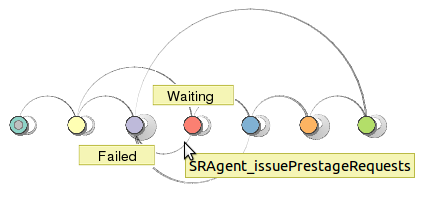
\includegraphics[width=0.9\linewidth,keepaspectratio=true]{./DiaGraphica.png}
\centering
\caption{CacheReplicaMem process visualization with DiaGraphica}
\label{fig:DiaGraphica}
\end{figure}%123478
\subsubsection{Model checking}
The default requirement specification language in the mCRL2 toolset
is the modal $\mu$-calculus \cite{ProcessesWithData}, extended with regular expressions and data.
Using the gained understanding of the system behavior, as well as the 
reported and anticipated problems, we formulated several requirements:

\lstset{tabsize=1,
  stringstyle=\ttfamily,
  caption={},
  %basicstyle=\small,
  breaklines=true,
  showstringspaces=false,
  morekeywords={tStaged,tDeleted,tFailed,tStageSubmitted,tNew,Done,Killed,MarkedForTermination,Running,JobInitialization}
 }
\renewcommand{\labelenumi}{\arabic{enumi}.}
\begin{enumerate}
\item Each task in a terminating state (``Failed'' or ``Staged'') is eventually removed from the system. (\textit{progress})

\item A deleted task will never be referenced for transition to any other state. (\textit{safety})

\item Once a job has been killed, it cannot resurrect and start running. (\textit{safety})

\end{enumerate}

Both requirements 1 and 2 were found to be violated, as can be seen from the traces (Fig.~\ref{fig:PropertyViolation}).
The race conditions manifest themselves in a few subtle interactions between the SMS storage and the agents.
In both cases, at step 4 the \textit{Stage Request Agent} issues prestage requests and 
as a result the CacheReplicas entries (second element of the State column) are updated to ``StageSubmitted''. Between the moment
that this agent has queried the storage and selected the corresponding Task to update to the same state,
to the point where the update is done (last step in both traces),
other agents may have monitored these replica records and updated
them to a new state, along with the associated Task. In practice, the manifestation
of such race conditions depends on the speed of the agents propagating the
state changes between the selection and update done by the \textit{Stage Request Agent}.
Such cases are nevertheless encountered in reality, when this agent
has large lists of records to process. This results in a deadlock situation, as 
the Task will have no further state updates made by other agents, since
from their perspective the state propagation is finished.

\begin{figure}[!tp]
\includegraphics[width=1\linewidth,keepaspectratio=true]{./PropertyViolation1.png}

\centering
\caption{Violation of requirements 1 (top) and 2 (bottom)}
\label{fig:PropertyViolation}
\end{figure}

Model checking with explicit state space generation was not a viable option for the WMS, due to its size (13 concurrent processes).
LTSmin's \cite{LTSmin} MPI version could not be used effectively here, because checking requirements on-the-fly
is currently not yet implemented, which thus forces generation of the (huge) overall state space.
We therefore resorted to using the LTSmin symbolic reachability tool which 
is almost instantaneous in traversing the state space, but does not
explicitly store it.
The tool has an option for tracking the occurrence of a certain specified action, and
reports the trace if such action is encountered during exploration. 
For this purpose, we extended the specification 
with a monitoring process which fires an error action if requirement 3 is
violated.

With respect to requirement 3, a counterexample showed that, when 
staging was involved in the workflow of a job, the callback from
the SMS was not properly handled.
It awakened the job immediately to a ``Waiting'' (and eventually ``Running'') state
even if it had been manually ``Killed'' 
(using DIRAC's command line API) by production managers meanwhile. Such zombie jobs
were discovered in the system on several occasions,
and with the model at hand it was easy to replay the behavior and localize the
problem. The longer trace is available at \cite{svn_mcrl2}. The implementation
was fixed to properly guard the callback against such transitions.


\section{Conclusions}
\label{sec:Section_5}
In this paper we have applied a formal methods approach for analyzing CERN's 
DIRAC grid system. 
We used two components as case studies: the Workload
Management and the Storage Management System, which are the driving force 
of DIRAC.
By creating an abstract model, simulating, visualizing, and model checking it with the mCRL2 toolset,
we were able to gain insight into the system behavior and detect critical
race-conditions and livelocks, which  
were confirmed to occur in the real system. 
Despite the continuous DIRAC development for 10 years, these problems 
were notoriously difficult to discover and trace, considering the number of concurrent components involved. 
With the model at hand, replaying
the traces and localizing the problems became much more straightforward, overcoming many limitations of
traditional testing techniques for large-scale distributed systems. Besides 
discovering behavioral problems, the 
model gives opportunities to analyze the system performance in the future.
By including quantitative metrics such as weights and probabilities in the generated LTSs,
we can compare the expected costs of certain ``what-if'' scenarios 
of interest, before implementing alternative designs.

The investment in writing an abstract model in a formal language 
pays off proportionally to the size (number of components) of the distributed system. 
This holds especially for grid systems where a large number of concurrent
 components of the same kind deliver the overall system functionality. 
Once becoming proficient with
the formal language notation, modeling such components is
reduced to reapplying similar abstraction rules.
Practitioners
of model checking have already built sufficiently mature tools
that can be utilized (almost) as blackboxes by more traditional
software developers, hiding the mathematical theories under
the hood. 
Although some domain-specific knowledge is always necessary,
the descriptive guidelines we have proposed for obtaining
an abstract model can be easily 
applied to other large-scale industrial systems of a similar nature.

\bibliographystyle{IEEEtran} 
\bibliography{myLibrary}

\end{document}


